\documentclass[beng,twoside,openright,logo]{infthesis}
\course{Software Engineering}
\project{Fourth Year Project Report}
\title{Improving feedback for a web-based marking system}
\author{Paul Thomson}
\abstract{This report discusses the work done towards improving the feedback supplied to users of the automated web-based marking system, Infandango. By applying machine learning methods to submission data recorded from students of a previous class, a model has been created which can predict a single score for the user which represents their progress so far. Through processes of optimisation and testing a Support Vector Machine has been chosen. This has been integrated with the Infandango system, providing a visual mechanism to display the cumulative feedback to the student.}

\begin{document}

\begin{preliminary}

\maketitle

\tableofcontents

\end{preliminary}

\chapter{Introduction}
\label{introduction}

\section{Infandango}
\subsection{Overview}
Infandango\cite{infandango_note} is an automated web-based marking system for student submitted programming exercises, currently only for the Java language. A student can view the list of warm-up, optional and core exercises and choose to submit a file for one of them. Jester is the testing daemon for Infandango which compiles and runs code inside a sandbox for security purposes. Between the web frontend and Jester there is a PostgreSQL database which stores the source code of each submission and the score information for each marked submission.

Each question has a label: {\bf warmup} questions are simple questions which can be skipped if the user feels confident, {\bf core} questions are questions which the user is highly encouraged to try and may affect the end coursework mark, and {\bf optional} questions are provided for particularly interested students.

\subsection{Current Use}
The system has been used with the first year Java programming course at the University of Edinburgh for a few years. The database information for these years has been kept and retains all the information about submissions: marks, submission time, number of resubmissions. The database for one year has been anonymised and made available for use in this project if necessary. Only one year is available because the questions have changed since previous years and therefore the data would be inconsistent with the current questions.

\subsection{Future Use}
Although Infandango was designed for a specific use, it has remained a general framework which can be adapted to have different content and is available as open-source software on bitbucket.org\cite{bitbucket}. Work is also currently being done to expand the number of possible languages that can be tested through Infandango\cite{bitbucket_james}.

\subsection{Current feedback}
The primary source of feedback in Infandango is displayed in Figure \ref{fig:currentfeedback}. Each submission is marked with a set of JUnit tests and typically one mark is given for each test that is passed. The marks are distributed such that at least 25 marks are available for each week. The fraction of passed tests to total tests is converted into a percentage and displayed on a red (0 - 40\%), orange (40\%-70\%) or green (70\%-100\%) background.
More general feedback is also available which displays similar information but the results are displayed by week rather than by question. 

\begin{figure}[h!]
\centering
\includegraphics[width=0.8\textwidth]{images/currentfeedback.png}
\caption{This is a cropped screenshot of what is displayed to the user for a given week in the current Infandango system}
\label{fig:currentfeedback}
\end{figure}

\section{Project Goals}
The general goal of this project was to improve the feedback for  Infandango. In order to achieve this, a list of objectives was created to facilitate the research, design and implementation of a suitable modification to the system:

\begin{enumerate}
\item Research and investigate current systems for providing automatic feedback to students. Examples where this feedback pertains to code are of particular interest.
\item Through evaluation of both the literature and the system choose an appropriate approach for providing feedback.
\item Implement the approach and then, when it is functional, integrate with the Infandango system.
\item Perform user evaluation of the completed work to determine any impact it has on the learning of the student
\end{enumerate}

Most of this report will be discussing how these objectives have been realised and the extent to which they have been completed will be discussed in Chapter \ref{conclusion}.

\chapter{Background}
\label{background}
\section{Infandango}
Infandango is an automated web-based marking system for student submitted programming exercises. A student can view the list of warm-up, optional and core exercises and choose to submit a file for one of them. This file is then compiled and tested by Jester in a sandbox. Between the web frontend and Jester there is a PostgresSQL database which stores which files have been submitted for which users and how these files performed on the JUnit tests.
\subsection{Current feedback}
The primary source of feedback in Infandango is displayed in Figure \ref{fig:currentfeedback}. Each submissions is marked with a set of JUnit tests and the fraction of these tests which are correct is displayed. This fraction is converted into a percentage and displyed on a green or red background depending on the value. %EPLXAINT HTIS LOL
More general feedback is also available which displays similar information but the results are displayed by week rather than by question. 

\begin{figure}[p]
\centering
\includegraphics[width=0.8\textwidth]{currentfeedback.png}
\caption{This is a crop of what will be displayed to the user for a given week}
\label{fig:currentfeedback}
\end{figure}

\section{Literature}
Khan Academy\cite{khan_site} is a website which provides users with online education material:
\begin{quote}
Our online materials cover subjects ranging from math and finance to history and art.  With thousands of bite-sized videos, step-by-step problems and instant data\cite{ka_faq}
\end{quote}
A blog post\cite{khan_blog} written by David Hu about Khan Academy demonstrates that different feedback measures can affect user performance significantly. The original Khan Academy system required a user to get 10 consecutive exercises of a certain type correct before they can be deemed proficient\footnote{A proficiency is earned when a user is deemed to be "proficient" at a certain kind of exercise} at that type of exercise. In an attempt to improve this system, a logistic regression model is used to calculate the probability that a user passes the next exercise successfully, with a threshold of 94\% representing the new proficieny level. Over a 6 day period 10\% of users tested the new method. Users of the new system earned 20.8\% more proficiences, attempted 15.7\% more exercises and required 26\% less exercises per proficiency. Hu summarises by saying the boost seems to come from allowing users to move on from exercises which they already proficient at, without requiring them to complete their streak thus wasting time on something they already understand.

\chapter{Design}
\label{design}
The literature has shown us that machine learning methods can be useful in generating feedback for students, and this can be combined with a visual display for intuitive understanding. The first design decision to be made is the language and libraries to be used when writing the program.
\section{Language and Tools}
Two languages are immediate possibilities for implementation: Java\cite{java_site} and Python\cite{python_site}. Java because I had the most experience with it and some parts of Infandango are written in Java. Most of Infandango was, however, written in Python with which I also had experience. Due to the emphasis the project has on machine learning, R\cite{r_site} was another approriate language. 
The final decision was to use Python with scikit-learn\cite{scikit_site} and pybrain\cite{pybrain_site} libraries: this provides the simplest integration with Infandango (since the parts with which this will need to be integrated are written in Python) and the libraries provide a variety of machine learning methods.

\section{Proposed Design}
Using the data from a previous year a model will be trained using machine learning methods. The model output a value which will be displayed somewhere in the Infandango system.
\subsection{Model}
The Infandango system is similar to the Khan Academy system and so the method Khan Academy uses is an approriate starting point. Infandango allows a user to submit many solutions for an exercise, and so does Khan Academy. However, there are two properties that distinguish Khan Academy from Infandango:

\begin{itemize}
\item For each exercise, the next solution submitted is for the same kind of question but the details are randomly generated %MAY NEED TO EXPLAIN THIS
\item A solution is a binary feature: correct or incorrect
\end{itemize}

This means a user can keep submitting solutions to an exercise even after they get one solution correct. However, in Infandango once a user gets 100\% there is no reason for the user to submit another solution because they have already perfected that exercise. The second difference means our data will be numerical instead of binary and this needs to be considered when designing the model.
The first difference is significant, and requires a change in granularity of the data: instead of measuring progress on a submission-by-submission basis, the focus should be on the final mark a user will achieve for an exercise. So instead of trying to predict the score for the next {\it submission}, try to predict the final score for the next {\it question}.

With an idea of how the model was going to work, some exploratory work was done on the data. Although users are encouraged to answer all questions, the do not receive marks directly for each question. This makes missing data a potential problem. Figure \ref{fig:missing_data} shows the submission rates for all the questions. It shows that submission rates can get as low as around 10\% for some questions. Figure \ref{fig:missing_data_core} shows the submission rates for only core questions. The submission rates are on average higher than for non-core questions. Combined with the fact that users are likely to have more motivation for core questions (since they potentially count towards their final mark) data from now on will only be considering core questions.

\begin{figure}[b!]
\centering
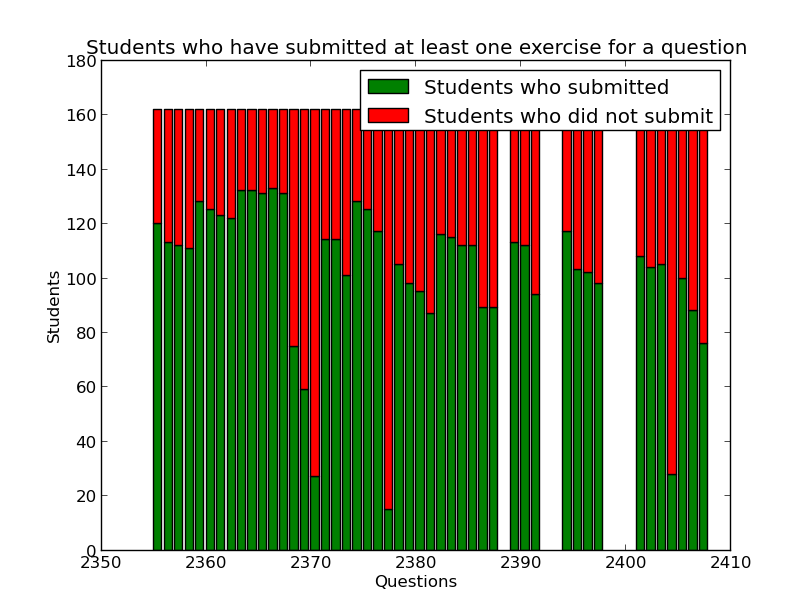
\includegraphics[width=0.8\textwidth]{images/missing_data.png}
\caption{Submission rates for all questions}
\label{fig:missing_data}
\end{figure}

\begin{figure}[b!]
\centering
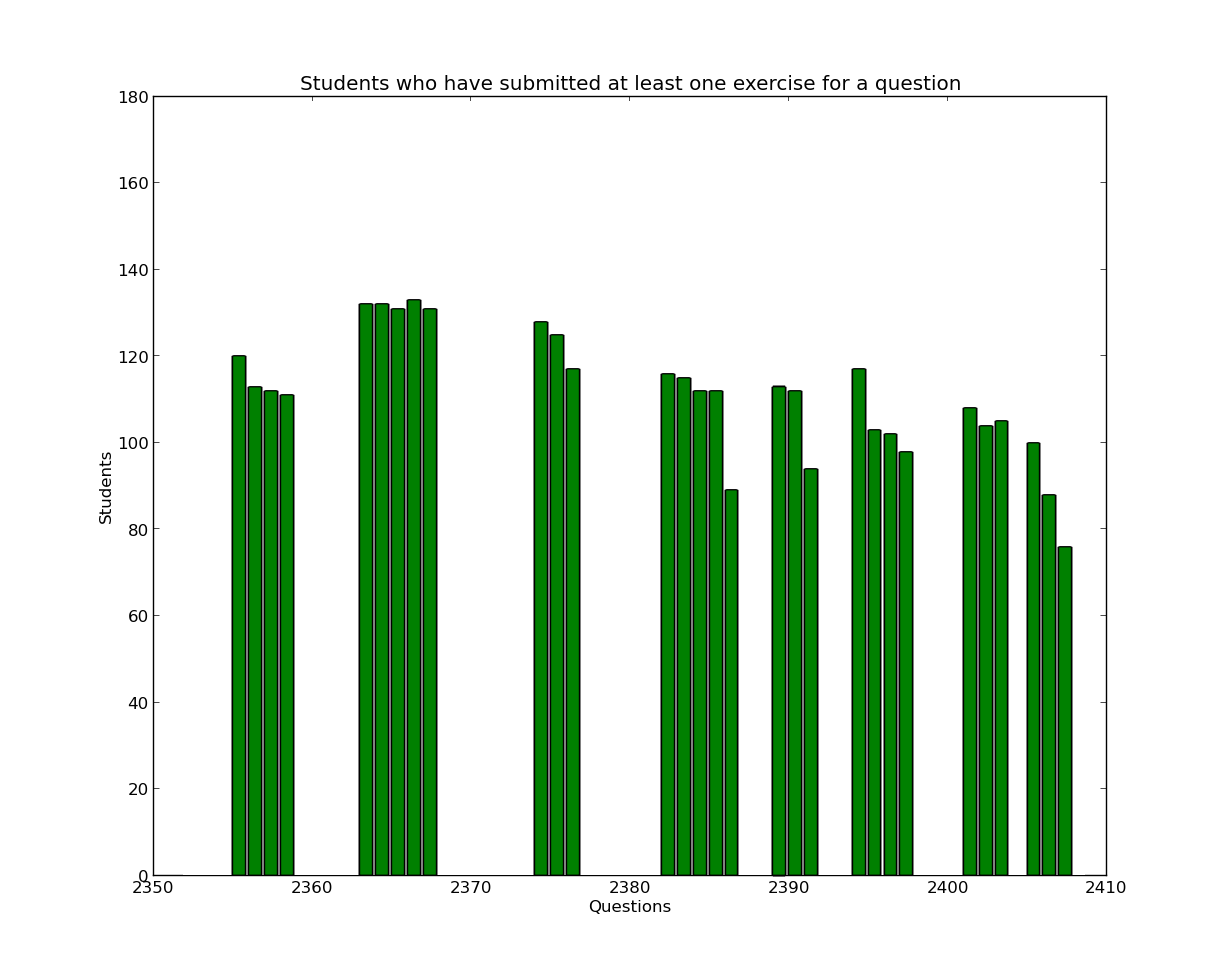
\includegraphics[width=0.8\textwidth]{images/missing_data_core.png}
\caption{Submission rates for only core questions}
\label{fig:missing_data_core}
\end{figure}

\begin{figure}[b!]
\centering
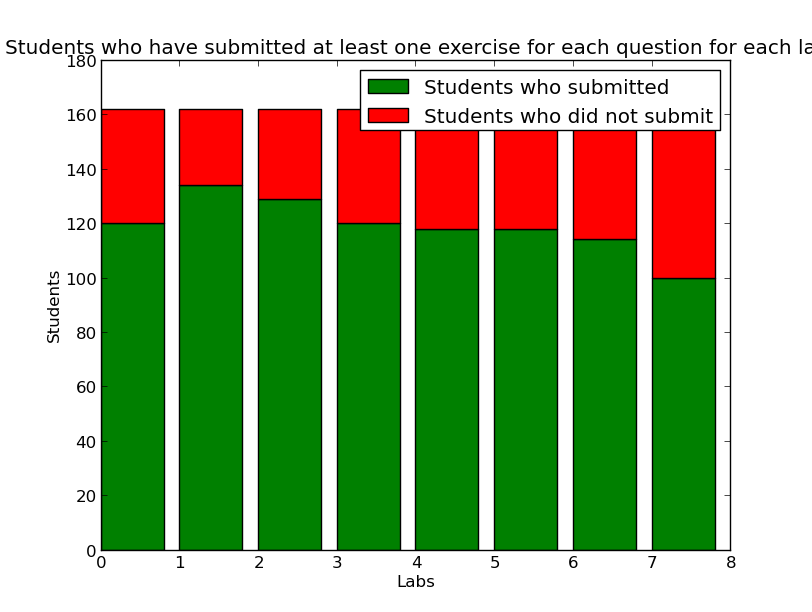
\includegraphics[width=0.8\textwidth]{images/missing_data_week_any.png}
\caption{Submission rates for at least one question per week}
\label{fig:missing_data_week_any}
\end{figure}

With the amount of missing data still being significant changing to yet another level of granularity was considered: predicting on a week-by-week basis. Using this method there could be a lot less missing data: take the average of all the questions for a week to get the score for that week. This means there will still be a data point for a student if they miss one question, and they would have to have no solutions for all questions in a week to get no score for a week. Comparing Figure \ref{fig:missing_data_week_any} to Figure \ref{fig:missing_data_core} a rise in the amount of data points can be seen. On average there is about 115 data points for a given week, and about 100 data points for a given question.

Although this does provide slightly higher yield there are disadvantages to predicting on a week-by-week basis:

\begin{enumerate}
\item It would take a week before there was even one data point to start giving feedback from
\item Feedback would only be updated weekly. After a student has been working on questions for a few days the feedback is likely to be outdated
\item A separate model would need to be trained for each week. To predict the score for week 3 you want to use two features: the score for weeks 1 and 2. For week 8 you would like to use all the available features: weeks 1 to 7. Having a variable number of features means having different models for each week
\end{enumerate}

Problems 1 and 2 are not really present if prediction is done question-by-question. Problem 3, however is still present: a new model needs to be trained for each question. A solution to this problem will be discussed later.

\subsubsection{Identity based features}
Starting with the Khan Academy model and adapting it based on Infandango and the available data a model can be proposed for Infandango: For each question, train a new model which takes all previous questions as input features. The model then tries to predict the score for that question.

\subsubsection{Moving Window}
Previously an assumption has been made: the identity of the question is necessary. While the identity of the question is likely to be important it is not necessary and removing this constraint allows a simple, singular alternative model to be proposed: The model always has N features and tries to predict the score of the N+1 question. For the simplicity of the following description N = 5 will be assumed.
There are 5 input features. The features will be decided based on their locality to the output feature: if we want to make a prediction for question 6 then the input features will be questions 1, 2, 3, 4 and 5. All the input features occur before question 6 because when a student is completing questions they are much more likely to do them in order, and so questions 7, 8 and 9 are not likely to present when making predictions. 
Although this approach does remove the significant information of the identity of the questions it is simple to implement and it also provides a lot more training data: There are 30 questions, and so using this approach for each student there would be 25 potential training examples. However, using the previous model there would only be 1 item for each model.



\subsection{Visualisation}


\section{Integration with Infandango}

\chapter{Model Selection}
\label{machinelearning}
In Chapter \ref{design} two data represenations were described which could be used in this scenario. To find out which data representation to use the first step is to choose some machine learning models to test on. Selecting the best model is a frequent problem which is still an active area of research. The first step is to use the labelled data to train and test various models. Given the tests results, a model can be selected. However, testing on the same data as was used in training can give results which will not be seen when the model is used on new data. Hence it is necessary to split the data into data to be used for training and data to be used for testing. This process is known as cross-validation and is the standard method of error prediction \cite{witten2011data}: the models are being validated against the test set. Cross-validation is most often performed more than once on the same dataset and the results are averaged. Doing so reduces the variance in the performance of the models.

After cross-validation has been performed each model has an error estimate. The final model is selected to have the lowest cross-validation error. However, due to the nature of cross-validation this error estimate may not be entirely accurate: we have deliberately chosen the model with the best cross-validation error, so it is possible that this error estimate is optimistic. To get the final error estimate the model is trained on all of the data used during cross-validation and tested on some separate, previously unseen data.

Although it cannot be certain that this model will perform best on new data, it is at least hoped that it will perform similarly to the final error estimate.

\section{Feature selection}
The first action to be taken when creating a model is to determine the features. The features determine the inputs to the model; the data which the model can use to learn and predict. Although the content of the inputs has been mostly decided already - the submission score - there is one aspect which has not been decided: how many scores should be considered? The moving window model must decide how large the window should be and the identity based model should consider the performance across the different model instantiations. The number of input features is a factor which will be discussed in the results section.

\subsection{Question Identity}
The two data representations differ on essentially one issue: is the question identity retained by the input features? One model says yes: retain the identities of the questions by assigning an index of the input vector to the same question each time (which means a new model must be created for each question). The second approach says no: create a moving window of input features from the questions immediately before the question we want to predict. This approach is quite wasteful: If the model is predicting the score for question 20 then it takes the results from questions 14 - 19 and ignores the other 13 questions. The model cannot take all the scores individually or it would be identical to the previous model, so a crude method of using all that extra data is to add an extra feature which is the numerical average of the unused data. By adding this feature to the moving window approach it remains simpler but doesn't completely ignore all the questions outside of the window.

\section{Preliminary models}
Most models will be chosen from the scikit-learn package except for Artificial Neural Networks (ANN) which are not present in scikit-learn. Pybrain provides the implementation of ANNs used here. As this is primarily an implementation issue this will be discussed further in Chapter \ref{implementation}.

Deciding on the models to use is a difficult process. However, since scikit-learn provides algorithms optimised for speed, most models are very quick to train and test. This allows the option of starting with a variety of models and then evaluating how they behave against each other. Depending on the type of data the expect and output, the models can be split into two different types: classifiers and regression models.

\subsection{Classifiers}
Classifiers attempt to identify the {\it class} an observation should be assigned to depending on the input features. A {\it class} is a discrete category, for example dog or cat. However what the models are trying to predict is the score of the next exercise which is a continuous value. To resolve this problem some sort of discretisation needs to be performed to change a percentage into a class. The granularity of this discretisation is important as it determines the amount of accuracy that can be achieved. 

A natural discretisation is already present in the current design: the visualisation on the webpage. The visualisation uses 9 blocks to display the score. For the sake of this application, any further accuracy would be lost when the information is displayed. So, in order to use classifiers on this problem, the output feature (the score we want to predict) will be discretised into one of 9 classes, distributed evenly over the range 0-100%.

\subsection{Regression}
Unlike the classifiers, no adaptations need to be made to the data before supplying it to the regression models sincer regressions output a continuous value like a percentage.

\subsection{Model definitions}

\paragraph*{Logistic Regression}
Although the name is misleading, this model is a classifier. It is originally a binary classifier but this problem has been formulated to use 9 classes. The multivariate implementation used by sci-kit uses the one-vs-all method. It can also use either L1 or L2 regularisation. The type of regularisation is the method used to calculate error, and so it defines how much a model is penalised for being wrong.
\subparagraph*{L1}
\begin{displaymath}
\left \|x  \right \|_{1} = \sum_{i}^{ } \left |x_{i}\right |
\end{displaymath}

\subparagraph*{L2}
\begin{displaymath}
\left \|x  \right \|_{2} = \sqrt{\sum_{i} \left |x^{2}_{i}\right |}
\end{displaymath}

\subsubsection{Linear Models}
The following models are all linear regressions: they expect the target value to be a linear combination of the input features. The differences between them occur in the constraints applied to the coefficients.

\paragraph*{Linear Regression}
This is the simplest linear model. It uses Ordinary Least Squares to estimate the coefficients of the input vector. This means it tries to minimise the residual sum of squares between the result given by the labelled data and the result predicted by the model.

\paragraph*{Ridge Regression}
This model adapts Linear Regression by adding to the minimisation value a penalty depending on the size of the coefficients. Scikit allows control of this penalty through the $\alpha$ parameter.

\paragraph*{LASSO}
This model applies a similar penalty as Ridge Regression except use the L1 norm instead. Scikit allows control of this penalty through the $\alpha$ parameter.

\paragraph*{Elastic Net}
Elastic Net combines the penalties of Ridge Regression and LASSO to provide a tradeoff between the two functionalities. This tradeoff can be controlled through the l1\_ratio parameter.

\paragraph*{Cross-validation}
Scikit also provides versions of these models which automatically apply cross-valdiation to determine the best values for their resepctive parameters.

\subsubsection{Support Vector Machines}
At the simplest level a Support Vector Machine (SVM) takes some input and assigns it to a binary class. At first this seems as linear as the previous models, but performing the {\it kernel trick} allows the SVM to deal with non-linear data. The choice of kernel can significantly affect the performance of the model. Two SVM implementations have been considered for this problem.

\paragraph*{Support Vector Classifier}
Scikit provides more than one Support Vector Classifier but SVC has been chosen due to its support of non-linear kernels. SVC uses the one-against-one approach for multiclass problems.

\paragraph*{Support Vector Regression}
SVR is scitkit's implementation of Support Vector Regression. It also supports non-linear kernels.

\subsubsection{Artificial Neural Network}
This model was chosen because it can model very complex relationships, which some of the previous models cannot. Like all models, it takes the input vector and produces an output. It does this by passing the input through a series of hidden layers. These hidden layers are created and calibrated during the training process. The library pybrain had to be used for this because scikit provides no implementation of an Artificial Neural Network.
Pybrain provides a wide variety of options, too many to be considered in this one implementation. Here are some of the options pybrain provides: Back propagation trainer, choice of hidden layer, choice of number of hidden units.

\section{Training and optimising}
Determining the best training methods and model parameters are tasks which can always be improved. Given the timescale of the project and the need to also integrate the model with the system, there are some model parameters and optimisation methods which have not been thoroughly investigated.

\subsection{K-fold cross validation}
%maybe discuss/reference a paper on cross-validation? this has already been discussed at beginning, maybe bring that part down here?
\section{Results}
Standard measurements of error (e.g. mean squared error) are dependent on whether the model is a classifier or a regressor: the mean squared error does not really make sense to a classifier, because it predicts a discrete class, not a continuous number. Similarly, using the frequency of an incorrect answer for a regressor does not make sense: it is highly unlikely to predict the exact continuous value. Therefore to allow comparison of the two types of models the output of the regressor is binned according to the available classes: the range 0-100 will be split into 9 equal ranges, {\it bins}. A percentage is converted into a class by determining the bin that contains it. Therefore binning the continuous values allows comparison with discrete values.
\paragraph*{Error function}
The function to determine the error will count the number of times the model predicts the incorrect class and divide this by the total number of examples. After multiplying this by 100 a percentage will be returned which represents the error rate.

\subsection{Linear Classifiers}
Due to the similarity of the Linear Regression based classifiers, these will be considered together and a representative model will be chosen based on the performances. As mentioned at the beginning of this chapter, both data representations have a variable number of input features and so accuracy will be discussed with respect to the number of input features.

\subsubsection{Optimisation}
The three variations of Linear Regression: Ridge, LASSO and Elastic Net each have parameters which can be tuned which affect regularisation. The method of choosing these parameters is similar to the method used to compared the models themselves.
Samples are taken from the range of possible values for each parameter (Elastic Net has two parameters, while Ridge and LASSO only have one). For each of these possible values, 10-fold cross validation is performed, with the average result being used as the error for that set of parameters.

\subsubsection{Optimisation Results}

\begin{figure}[h!]
\centering
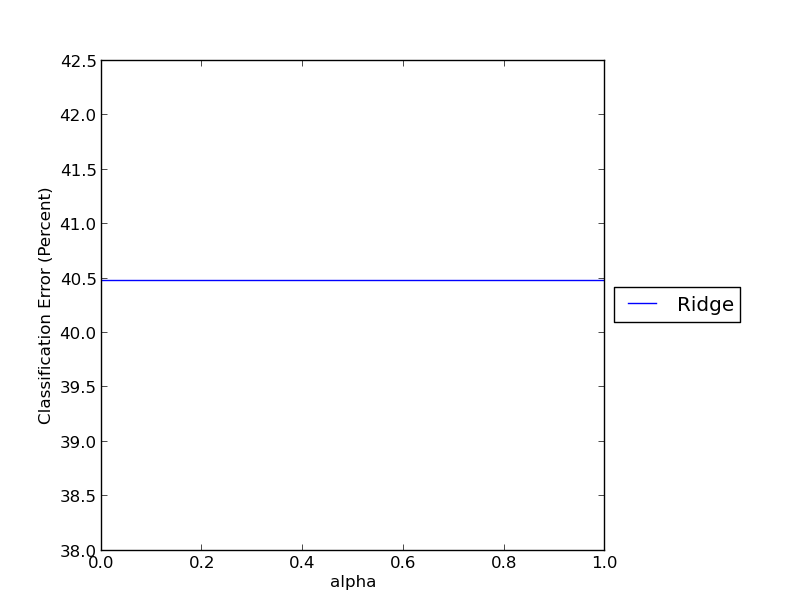
\includegraphics[width=0.8\textwidth]{images/ridgealpha.png}
\caption{The effect on error rate of changing the alpha parameter on Ridge Regression}
\label{fig:ridgealpha}
\end{figure}

\begin{figure}[h!]
\centering
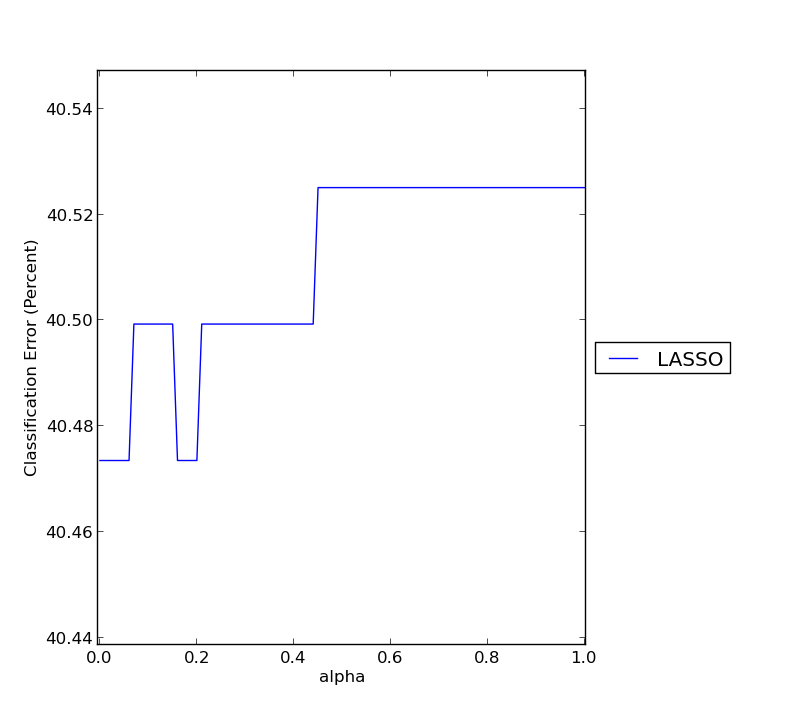
\includegraphics[width=0.8\textwidth]{images/lassoalpha.png}
\caption{The effect on error rate of changing the alpha parameter on LASSO}
\label{fig:lassoalpha}
\end{figure}

\begin{figure}[h!]
\centering
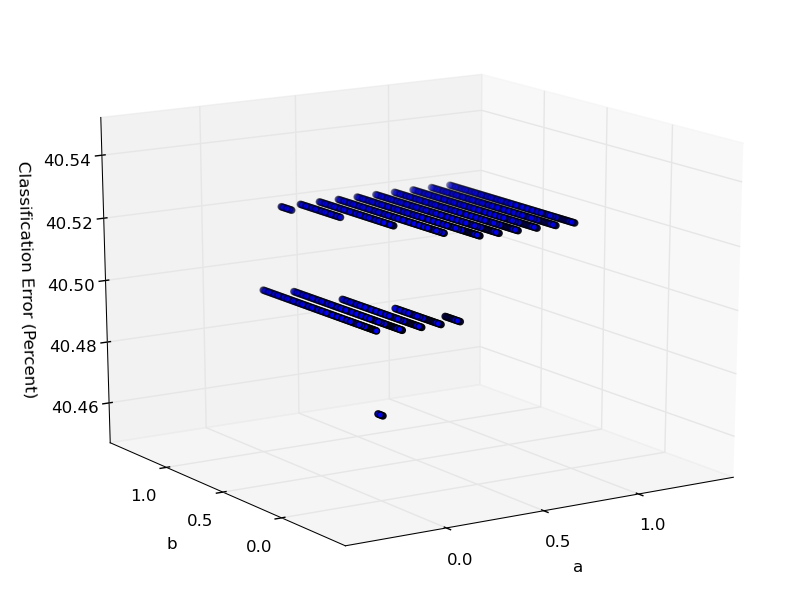
\includegraphics[width=0.8\textwidth]{images/elasticnetab.png}
\caption{The effect on error rate of changing the a and b parameters on Elastic Net}
\label{fig:elasticnetab}
\end{figure}

Figures \ref{fig:ridgealpha}, \ref{fig:lassoalpha} and \ref{fig:elasticnetab} show that none of the parameters have a drastic effect on the error rate of the models. The results for Ridge Regression show no change in the performance of the classifier when changing the parameter, alpha. The following values will be used for these models from now on: Ridge Regression: alpha = 1; LASSO: alpha = 1; ElasticNet: a = 0, b = 0.

\subsubsection{Comparing the Linear Models}
Using the cross-validation method described previously, the 4 different linear models were trained with the parameters discovered via optimisation.

\begin{figure}[h!]
\centering
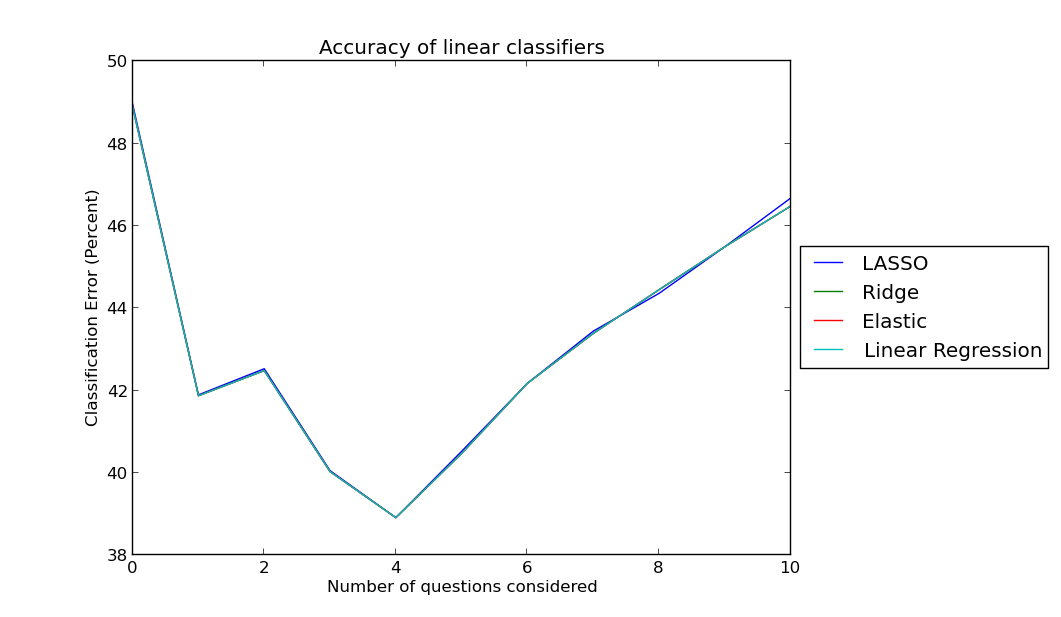
\includegraphics[width=0.8\textwidth]{images/linearmodelsmovingwindow.png}
\caption{The error rates for linear models using the moving window data representation}
\label{fig:linearmodelsmovingwindow}
\end{figure}

\begin{figure}[h!]
\centering
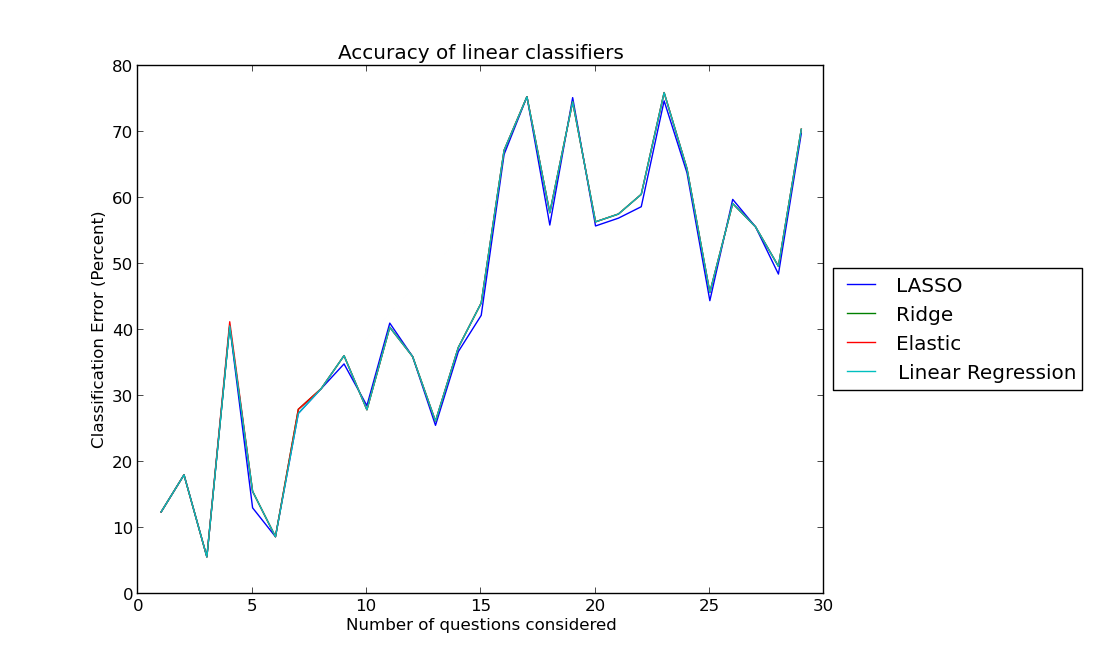
\includegraphics[width=0.8\textwidth]{images/linearmodelsidentified.png}
\caption{The error rates for linear models using the identity based data representation}
\label{fig:linearmodelsidentified}
\end{figure}

Figure \ref{fig:linearmodelsmovingwindow} shows that the performance of the models depends largely on the size of the moving window. For these models the lowest error rate is acheived when the window is of size 4. For this data, the error rate increases as more questions are considered which is at first unexpected: if the model knows more about the previous questions then it should be able to have a more accurate prediction. 

One possible explanation is that the new data is not as relevant. Questions in Infandango are grouped - though not strictly - by the type of the questions: a question is likely to build on knowledge of the previous question. For this reason, results of questions within the same locality are likely to be useful in predicting the results of other questions in the same locality. As this locality is increased the questions become less likely to be relevant to the target question. Not only will these questions add little information, they may also obscure the relevant information from the training algorithms.

Another potential reason for the increasing error rate is that as the window size increases there is less usable data, per observed datapoint, to train on. This is shown in Figure \ref{fig:movingwindowdata}. Less training data means the algorithms have less time to adjust the weights used to predict scores.

\begin{figure}[h!]
\centering
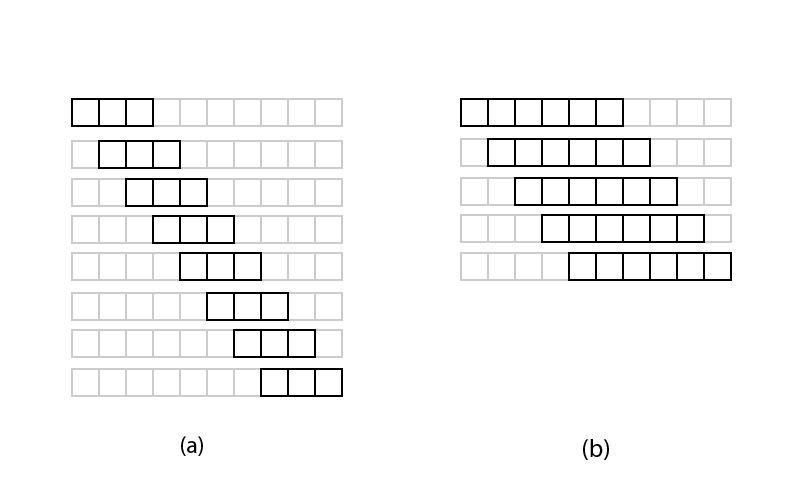
\includegraphics[width=0.8\textwidth]{images/movingwindowdata.png}
\caption{(a) shows how much data can be used with a moving window of size 3 (8 pieces of data), (b) shows the same for a window of size 6 (5 pieces of data).}
\label{fig:movingwindowdata}
\end{figure}

Figure \ref{fig:linearmodelsidentified} shows the lowest error rate when considering 4 questions - interestingly this is the same as the moving window approach. The error rate generally increases as more questions are considered although the behaviour is erratic.
The increase in error rate might be attributed to one of the reasons for the increase in error rate of the moving window approach: as more questions are considered, less of them are relevant.

One factor which might account for both the increase in the error rate and the erratic behaviour is that, in general, this approach will have much less training data than the moving window approach.

As seen in figure \ref{fig:movingwindowdata} the moving window approach can, for one model, train multiple times on the same piece of data. The reason it can do this is that it does not need to consider the identity of the question. However, retaining the identity is exactly how the identity based model differs from the moving window model. For this reason it can only train once on each piece of data, whereas the moving window approach might receive 20 pieces of data from one observed item.

\subsubsection{Conclusion of Linear Models}
One interesting feature of the results so far is that all the linear models behave very similarly on both data representations. Since the graphs do not give any obvious indications of the best model, the averages have been calculated for each model for each data representation, shown in Table \ref{table:linearmodelsaverages}.

The lowest average is shared by Linear Regression, Ridge Regression and Elastic Net. Since Ridge Regression and Elastic Net are Linear Regression with added regularisation, the simpler option will be chosen. Therefore the best Linear model is Linear Regression using the Moving Window approach.

\begin{figure}[h!]
\centering
\begin{tabular}{l || l | l}
Models & Moving Window & Identity based \\ \hline \hline
Linear Regression & 43.1508290455 & 44.066091954 \\ \hline
Ridge Regression & 43.1508290455 & 44.0876436782 \\ \hline
LASSO & 43.1844660458 & 43.5512452107 \\ \hline
Elastic Net & 43.1508290455 & 44.1091954023 \\ \hline
\end{tabular}
\caption{Average error rate for the linear models on two different data representations}
\label{table:linearmodelsaverages}
\end{figure}

\subsection{Support Vector Machines}
A Support Vector Machine is an algorithm that attempts to find a maximum margin hyperplane, which is defined by the {\it support vectors}: the vectors which lie the same distance (margin) away from the hyperplane. This margin is maximised so that the hyperplane lies as far away from each class as possible. A new data point is labelled depending on what side of the hyperplane it lies on. Figure \ref{fig:hyperplane} shows an example hyperplane on two dimensional data, although SVM can work on any number of dimensions.

\begin{figure}[h!]
\centering
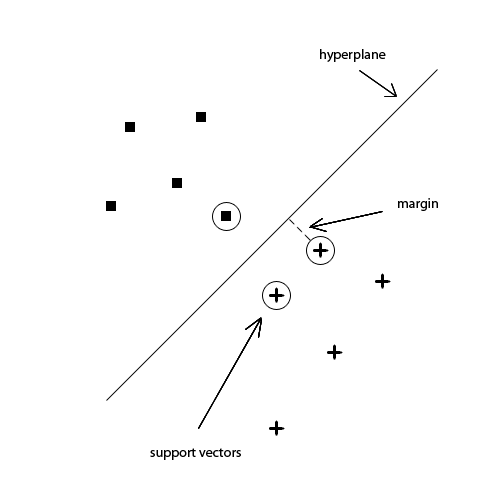
\includegraphics[width=0.8\textwidth]{images/hyperplane.png}
\caption{A maximum margin hyperplane that separates two classes in a two dimensional space}
\label{fig:hyperplane}
\end{figure}

\subsubsection{Kernel Functions}
The simplest, linear Support Vector Machines attempt to find a maximum margin hyperplane using a method which requires calculating the dot product between vectors. In the linear case, the standard dot product is enough to allow the data to be separated. However, if the data is more complex it may not be the approriate function to use. Changing this dot product to be some other function (which must take two vectors and return a scalar value) is what is known as the "kernel trick". The candidate functions are known as kernel functions, and allow for the SVMs to be applied to non-linear data. 

\subsubsection{Optimisation}
Scikit provides 4 preset kernel functions: linear, polynomial, rbf (radial basis function) and sigmoid. In the case of polynomial and sigmoid kernels, an additional parameter, "degree", allows the specification of the degree of the kernel. An appropriate way of finding good values for this parameter is to start at 1, and increase until the estimated error ceases to improve \cite{witten2011data}. 

\begin{figure}[h!]
\centering
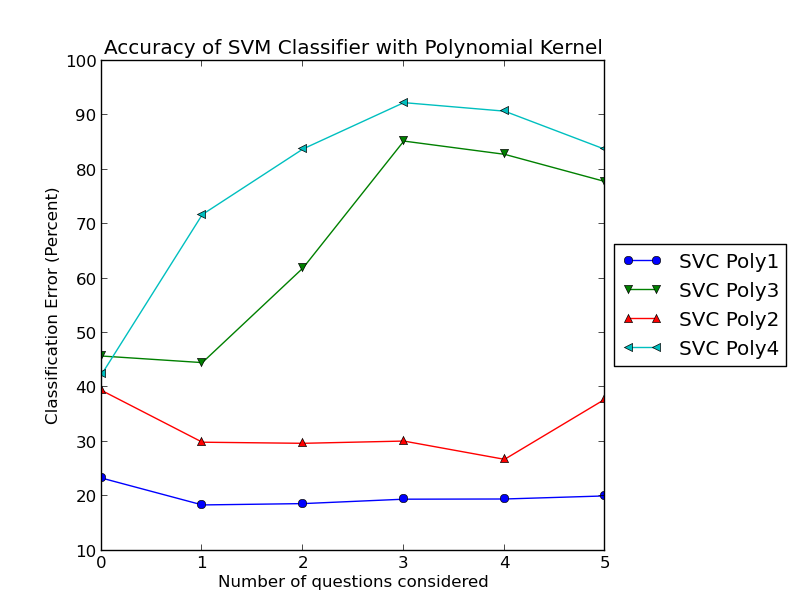
\includegraphics[width=0.8\textwidth]{images/svcpoly.png}
\caption{The performance of a SVM classifier using a polynomial kernel with different degree values}
\label{fig:svcpoly}
\end{figure}

\begin{figure}[h!]
\centering
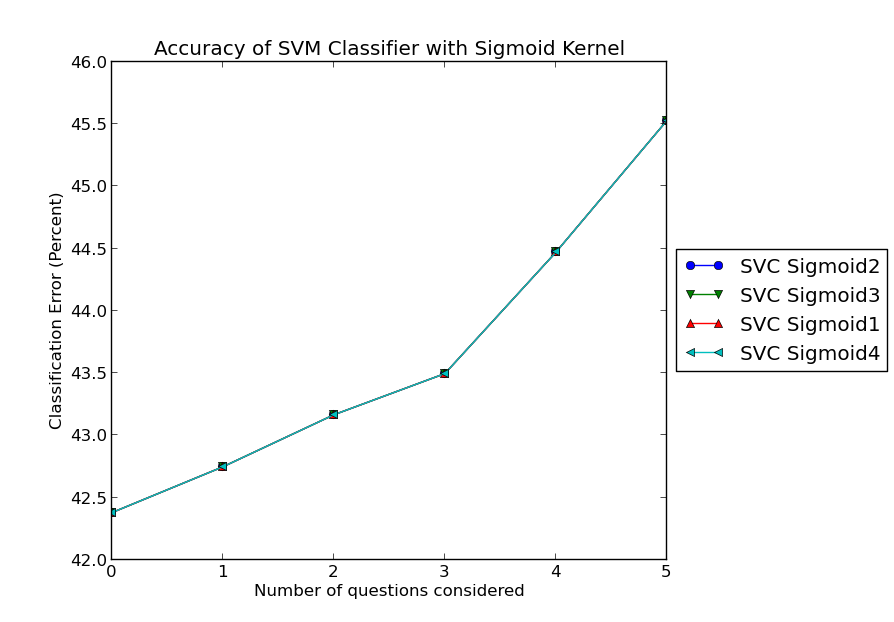
\includegraphics[width=0.8\textwidth]{images/svcsigmoid.png}
\caption{The performance of a SVM classifier using a sigmod kernel with different degree values}
\label{fig:svcsigmoid}
\end{figure}

\begin{figure}[h!]
\centering
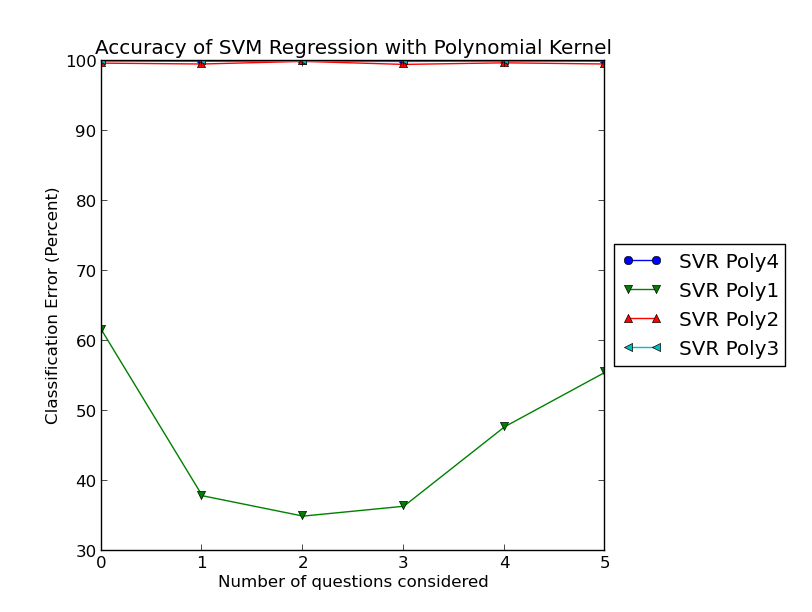
\includegraphics[width=0.8\textwidth]{images/svrpoly.png}
\caption{The performance of a SVM regression using a polynomial kernel with different degree values}
\label{fig:svrpoly}
\end{figure}

\begin{figure}[h!]
\centering
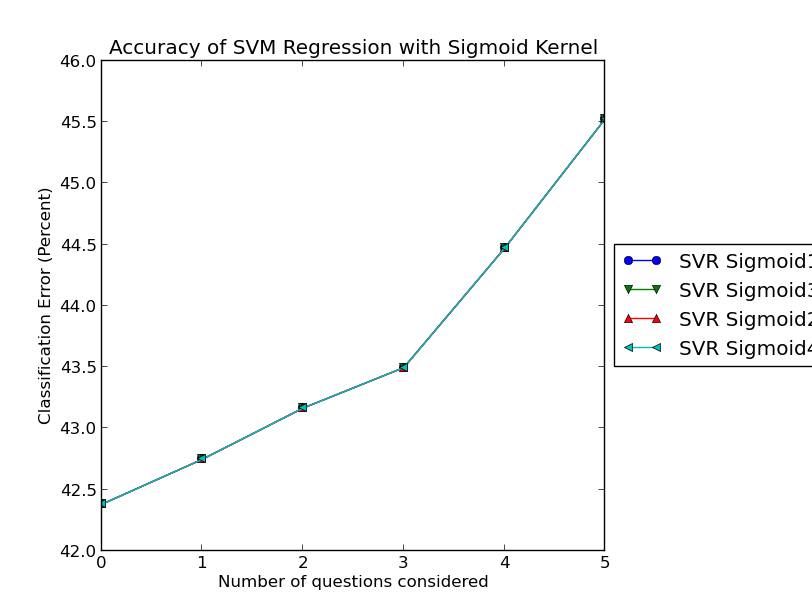
\includegraphics[width=0.8\textwidth]{images/svrsigmoid.png}
\caption{The performance of a SVM regression using a sigmoid kernel with different degree values}
\label{fig:svrsigmoid}
\end{figure}

Figures \ref{fig:svcsigmoid} and \ref{fig:svrsigmoid} show the effect of changing the degree of the sigmoid kernel. In both cases, changing the degree has no effect on the performance of the model. Figures \ref{fig:svcpoly} and \ref{fig:svrpoly} show the effect of changing the degree of a polynomial kernel. Here, changing the degree has a significant affect. In both cases the best value is 1, with the other values performing significantly worse.

\subsubsection{Results}
With the optimisations completed, the different models could be compared against each other. Figure \ref{fig:svmsmovingwindow} and Table \ref{table:svmsmovingwindowaverages} show the results for the moving window approach. Figure \ref{fig:svmsidentified} and Table \ref{table:svmsidentityaverages} show the results for the identity based approach. 
The moving window approach has three similarly high performing models: SVC Linear, SVC Poly, SVC RBF. These models show a very similar performance in the identity based approach, although as with all models their performance is more erratic.

\begin{figure}[h!]
\centering
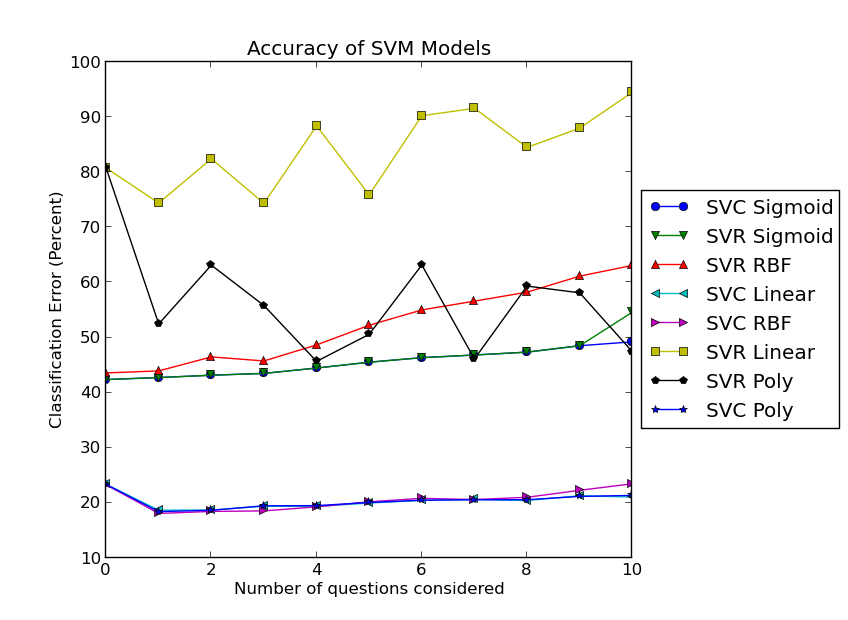
\includegraphics[width=0.8\textwidth]{images/svmsmovingwindow.png}
\caption{The performance of various SVM models}
\label{fig:svmsmovingwindow}
\end{figure}

\begin{figure}[h!]
\centering
\begin{tabular}{l || l }
Models & Average Error \\ \hline \hline
SVC Linear & 20.3041791411 \\ \hline
SVC Poly & 20.3313952482 \\ \hline
SVC RBF & 20.5499438422 \\ \hline
SVC Sigmoid & 45.4603396387 \\ \hline
SVR Sigmoid & 45.9489389873 \\ \hline
SVR RBF & 52.2508272032 \\ \hline
SVR Poly & 56.6047985482 \\ \hline
SVR Linear & 84.1041319495 \\ \hline

\end{tabular}
\caption{Average error rate for SVMs using the moving window approach}
\label{table:svmsmovingwindowaverages}
\end{figure}


\begin{figure}[h!]
\centering
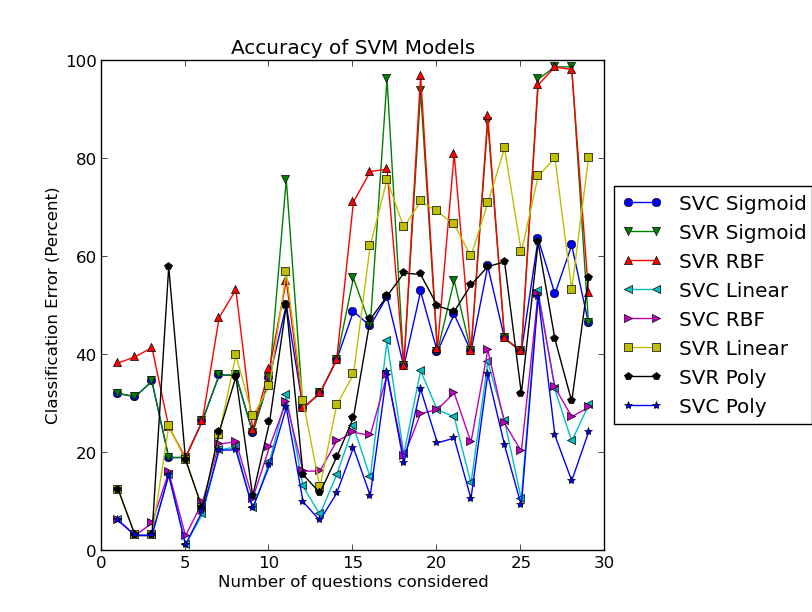
\includegraphics[width=0.8\textwidth]{images/svmsidentified.png}
\caption{The performance of various SVM models}
\label{fig:svmsidentified}
\end{figure}

\begin{figure}[h!]
\centering
\begin{tabular}{l || l }
Models & Average Error \\ \hline \hline
SVC Linear & 20.5459770115 \\ \hline
SVC Poly & 17.8424329502 \\ \hline
SVC RBF & 22.3659003831 \\ \hline
SVR Poly & 35.5555555556 \\ \hline
SVC Sigmoid & 40.6082375479 \\ \hline
SVR Linear & 46.1206896552 \\ \hline
SVR Sigmoid & 49.8970306513 \\ \hline
SVR RBF & 53.43151341 \\ \hline

\end{tabular}
\caption{Average error rate for SVMs using the moving identity based approach}
\label{table:svmsidentityaverages}
\end{figure}

\subsubsection{Conclusion}
3 models perform very similarly on both approaches which makes choosing between them more difficult, although it is at least clear that it should be a classifier. Due to having the lowest combined average, the model chosen as the best SVM is classification with a polynomial kernel of degree 1.

\subsection{Artificial Neural Network}
The ANN implementation used for this project is provided by the Pybrain library. An ANN takes the inputs, passes all the inputs to each unit in a "hidden" layer and the outputs of each unit in the hidden layer are passed to the output units. The units in the hidden layer are artificial neurons and can be of various types. For example, a neuron could be the weighted sum of the inputs. Figure \ref{fig:nn} shows how an ANN suitable for this problem might look. 

\begin{figure}[h!]
\centering
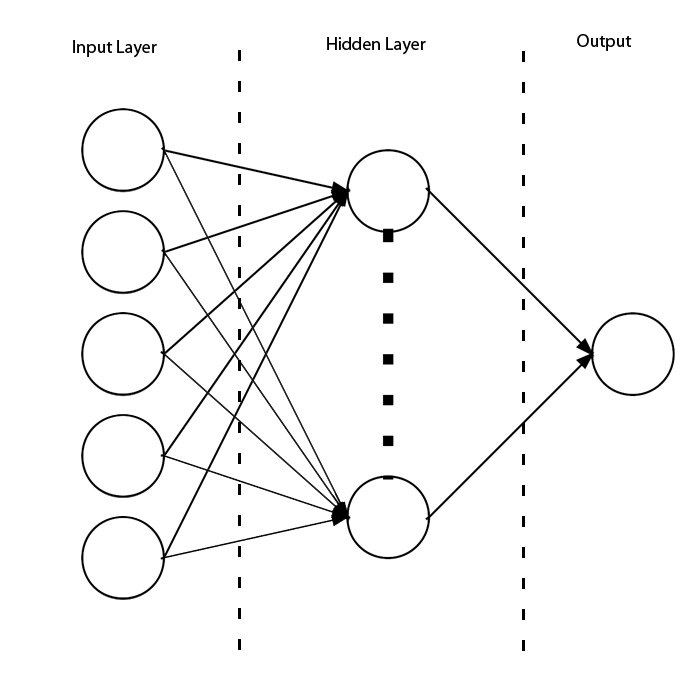
\includegraphics[width=0.8\textwidth]{images/nn.png}
\caption{The topology of an Artificial Neural Network with 5 inputs, one hidden layer with an unspecified number of units and one output unit.}
\label{fig:nn}
\end{figure}

Since Pybrain is a library which focuses specifically on ANNs it has even more customisation than scikit-learn does for its models. The two parameters investigated are the type of units in the hidden layer and the number of units in the hidden. Changing these parameters allows the model to be as complex as the problem requires.

\subsubsection{Optimisation}
Pybrain provides many types of hidden layer, including GaussianLayer, LinearLayer, SigmoidLayer and TanhLayer. Due to technical issues which will be discussed in Chatper \ref{implementation} the layers chosen were SigmoidLayer and TanhLayer.

\subsubsection{Results}
Figure \ref{fig:nnall200} shows how different parameters effect the error of the model. Both models perform similarly except the TanhLayer has a large drop in error rate with 130 hidden units.

\begin{figure}[h!]
\centering
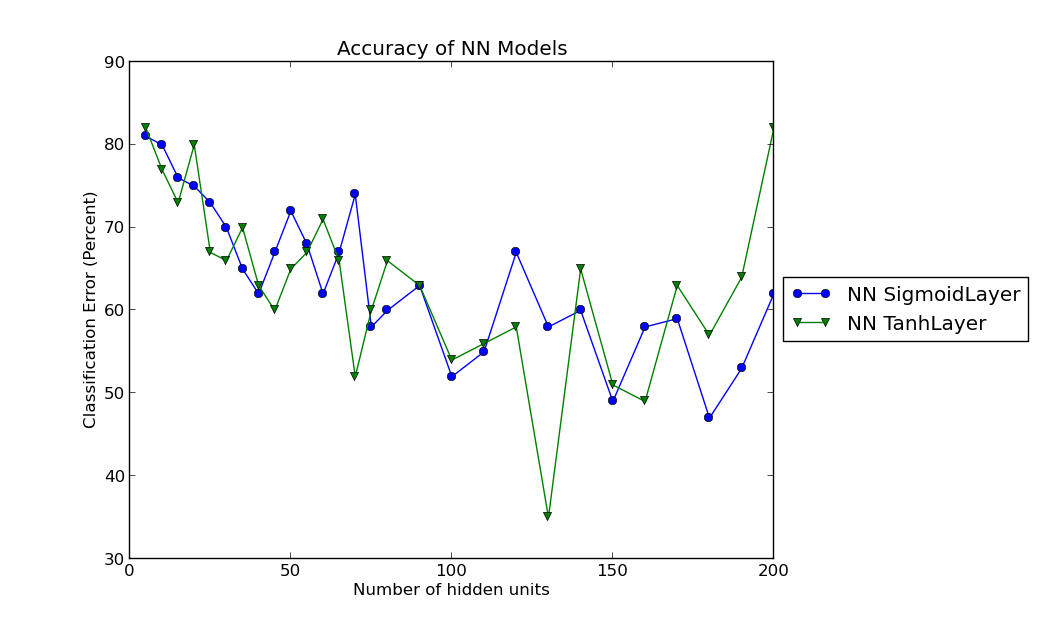
\includegraphics[width=0.8\textwidth]{images/nnall200.png}
\caption{The effect of changing the number of hidden units on Neural Networks with two different hidden layer types.}
\label{fig:nnall200}
\end{figure}

\subsubsection{Conclusion}
There is little to choose between both models, as both have the same general trend and neither performs consistently better than the other. Although it is possibly an anomaly, the model chosen is Artificial Neural Network with Sigmoid squashing function as the hidden layer type with 130 hidden units.

\subsection{Final Model Selection}
The final task is to choose the model that is going to be used in the system. To do this, each of the models are trained and tested on both data representations. Each model uses the parameters determined through optimisation.

\begin{figure}[h!]
\centering
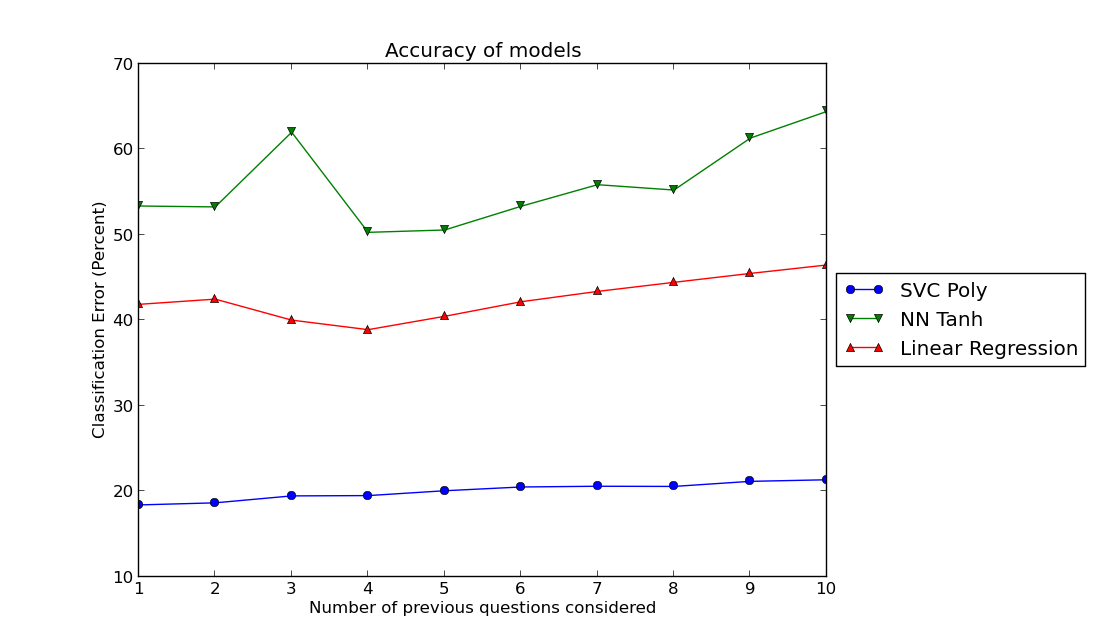
\includegraphics[width=0.8\textwidth]{images/movingwindowfinal.png}
\caption{The performance of the optimised models using the moving window approach}
\label{fig:movingwindowfinal}
\end{figure}

\begin{figure}[h!]
\centering
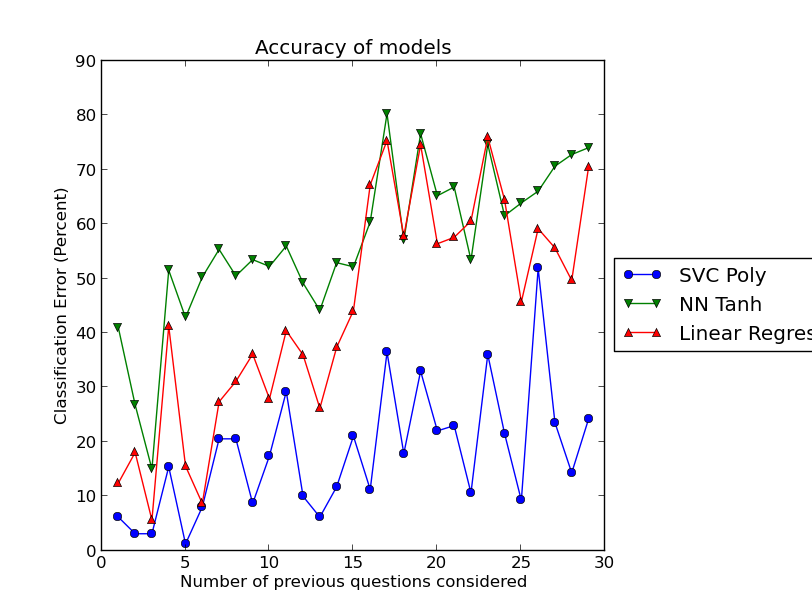
\includegraphics[width=0.8\textwidth]{images/identifiedfinal.png}
\caption{The performance of the optimised models using the identity based approach}
\label{fig:identifiedfinal}
\end{figure}

Figure \ref{fig:movingwindowfinal}

\chapter{Implementation}
\label{implementation}
\section{Introduction}
In the previous chapter a model was chosen from many other models by measuring the error rates. Graphical mockups were created for the visual design of the feedback. This chapter will explain the process through which these two elements were implemented. The implementation required understanding of how the Infandango system works, specifically how it renders webpages. The completed system gives a visual display for the predicted score retrieved from the model.

\section{Language and Tools}
Two languages are immediate possibilities for implementation: Java\cite{java_site} and Python\cite{python_site}. Java was considered because I had the most experience with it and some parts of Infandango are written in Java. Most of Infandango is, however, written in Python with which I also had experience. Due to the emphasis the project has on machine learning, R\cite{r_site} was another approriate language.

The final decision was to use Python with scikit-learn\cite{scikit_site} and pybrain\cite{pybrain2010jmlr} libraries: this provides the simplest integration with Infandango (since the parts with which this will need to be integrated are written in Python) and the libraries provide a variety of machine learning methods.

\section{Visual Design}
The final design is relatively simple and since the system is web based, web technologies like Javascript and CSS were considered. The choice between implementation strategies was based on the ease of integration with Infandango: although Infandango does already use Javascript like the Scriptaculous library\cite{scriptaculous_site}, CSS is more heavily used. For example, the lab exercise page Infandango displays a single score for an exercise with a background colour determined by the score (red for a bad score, green for a good score). Pure CSS is used here where Javascript could also have been, and so a similar CSS based approach was used for the visualisation.

\section{Prediction Model}
Most of the code used to choose the model in Chapter \ref{machinelearning} can be used here: loading data, parsing data, training the model and performing a prediction. The final remaining step is allowing Infandango access to the model, a problem for which two solutions were immediately considered.

The first solution is to load the data and train the model when Infandango first starts. This object would then passed around to the appropriate place, staying in memory and being used whenever it is needed. Some problems with this architecture are:

\begin{enumerate}
\item It makes changing the model during runtime more or less impossible without restarting Infandango.
\item The data used for training would also need to be stored somewhere, which could require a separate database running alongside the active database.
\item It could potentially cause some coupling between the code used for training the model and the Infandango startup procedure, making future adaptations more difficult.
\end{enumerate}

The second solution is training the model beforehand and storing/loading this model to be used when necessary. A problem with this approach is that loading the model must occur during runtime which could potentially slow the loading speed of the web page. However, this approach does overcome some of the problems of the previous approach: 

\begin{enumerate}
\item The model can be changed easily, providing it uses the same loading interface.
\item Only the model needs to be stored, not all the data used for training.
\item Any model and training procedure can be used, as long as the same call can be made to make a prediction.
\end{enumerate}

The final implementation uses the second solution: training procedures discussed in chapter \ref{machinelearning} to train the model and serialises it using the standard python module, pickle\cite{pythonpickle_site}.

\section{System Integration}
When a page is requested the request is passed to Django. Django will then be given the necessary information from the database to fulfil this request. Each page has methods which generate dynamic content for that page (e.g. retrieve information from the database). Since the progress bar is attaching to the sidebar --- an item which appears on every page --- then manually adding the prediction code to every page would take time, would be very difficult to change and is generally undesirable. Instead, Django offers ``Context Processors''\cite{django_cp} which is a way of hooking methods into the call that loads every page, allowing this content to be used by any page without telling every page explicitly. 

For example, the following function is a current context processor in Infandango.

\begin{verbatim}
def labSheetListMenu(request):
  return {"lab_sheets": LabSheet.objects.all() }
\end{verbatim}

This first half, {\tt"lab_sheets"}, is the name webpages can use to refer to the object. The second half, {\tt LabSheet.objects.all()}, is the object referred to by the first half, and is a database request. This context processor allows all webpages to access the list of lab sheets, which is needed for the navigation sidebar.

\section{Technical Issues}

\subsection{Neural Network Hidden Layers}
Although Pybrain provides many different types of hidden layers only two were used: Sigmoid and Tanh. All attempts with other layers would lead to an error due to an overflow occuring, perhaps caused by the amount of data used. These errors may not happen for Sigmoid and Tanh layers as they are squashing functions.

\subsection{Slow Neural Networks}
The Pybrain library was used due to it being written in Python and its ease of use. However, a factor not fully considered at first was the speed. Although the speed is not a problem when performing a prediction, it becomes an impediment when performing optimisation and cross-fold validation. In an effort to mitigate this problem, the arac library\cite{arac_site} was used, in conjunction with Pybrain to provide fast implementations of the neural networks provided by Pybrain. Due to the alpha state of the project some additional time was needed after installation in order to debug the library, but a working solution was found which on average reduced neural network training time by 50\%.

\section{Conclusion}
Using the Django context processor functionality a function is hooked into every web page request. This function de-serialises the trained model and uses it to provide a prediction based on previous exercise submissions. This prediction is used to determine the colours which will be displayed in each box and this is facilitated through Django. Figure \ref{fig:contextprocessor} shows the control flow of this process. This concludes the implementation of the feedback mechanism, and Figure \ref{fig:finalfeedback} shows a screen capture of the feedback mechanism in Infandango.

\begin{figure}[h!]
\centering
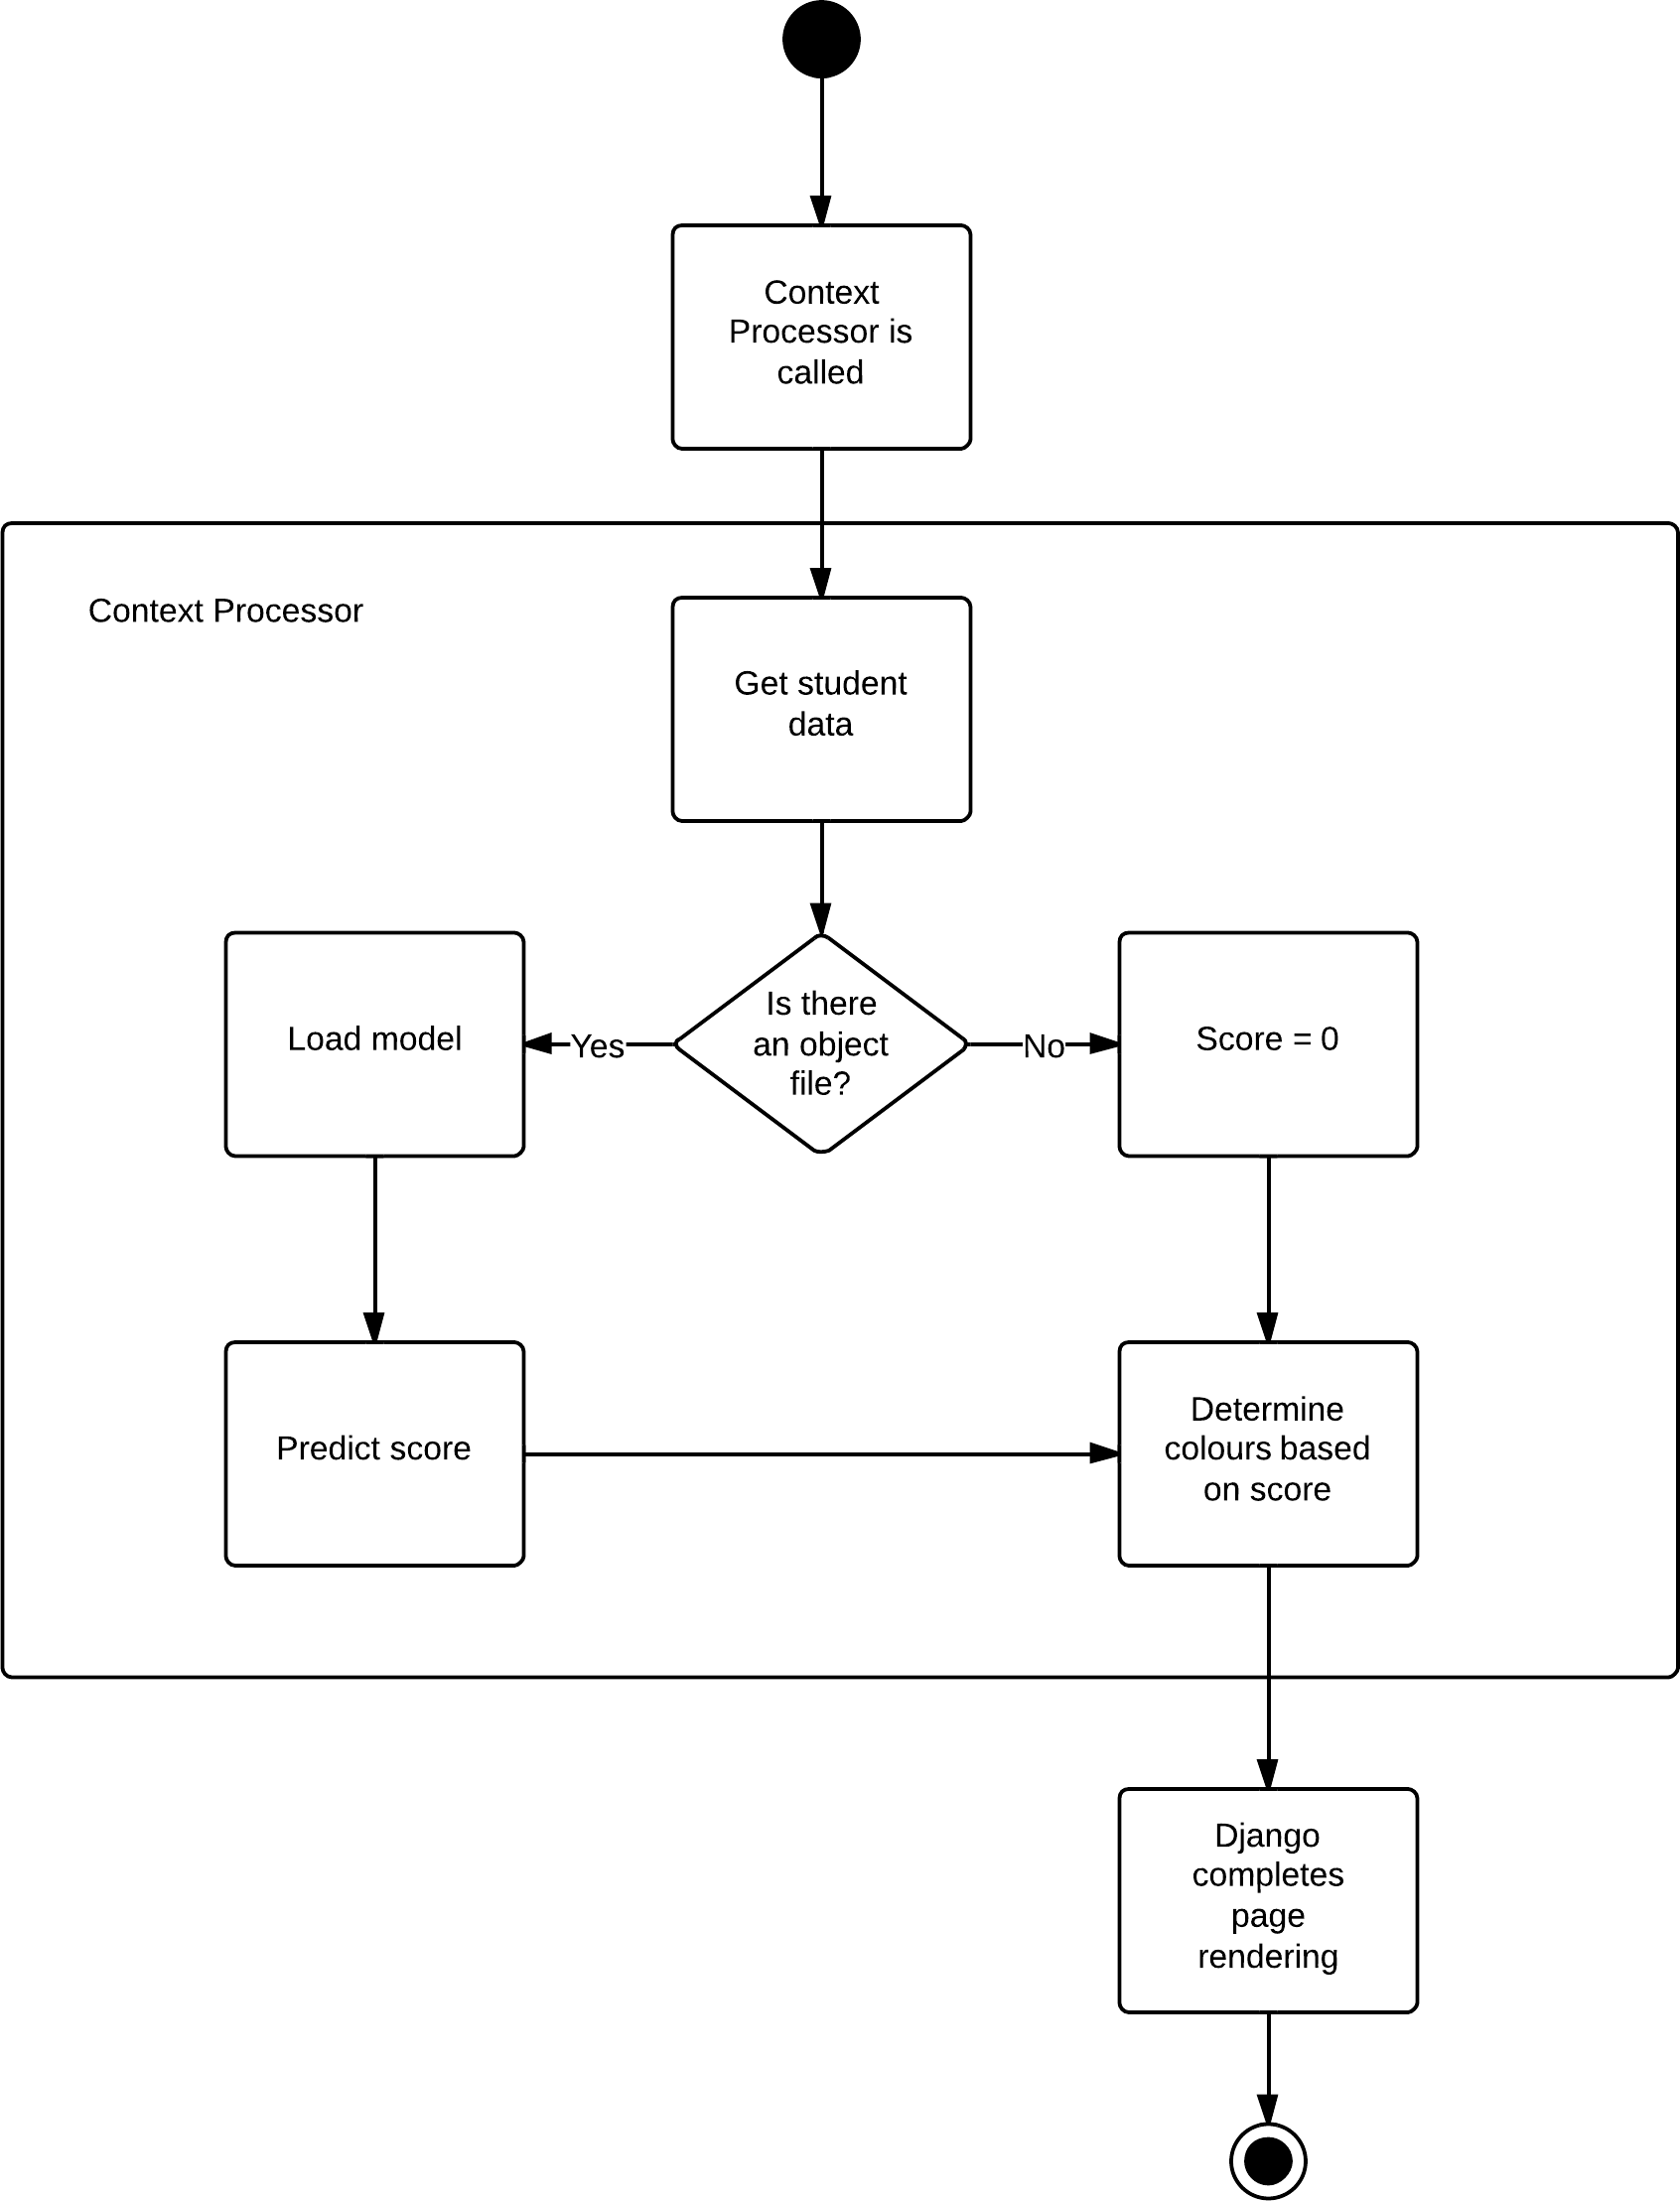
\includegraphics[width=0.8\textwidth]{images/contextprocessor.png}
\caption{A flowchart of the context processor function and how it interacts with Django}
\label{fig:contextprocessor}

\begin{figure}[h!]
\centering
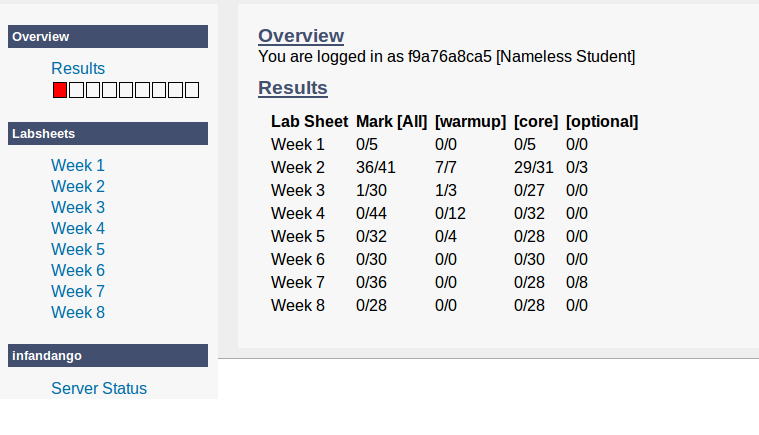
\includegraphics[width=0.8\textwidth]{images/finalfeedback.png}
\caption{A screenshot of what a user might see using the new feedback mechanism in Infandango}
\label{fig:finalfeedback}
\end{figure}

\chapter{Evaluation}
\label{evaluation}

\chapter{Conclusion}


\appendix
%\chapter{K-means Clustering}

\begin{figure}[h!]
\centering
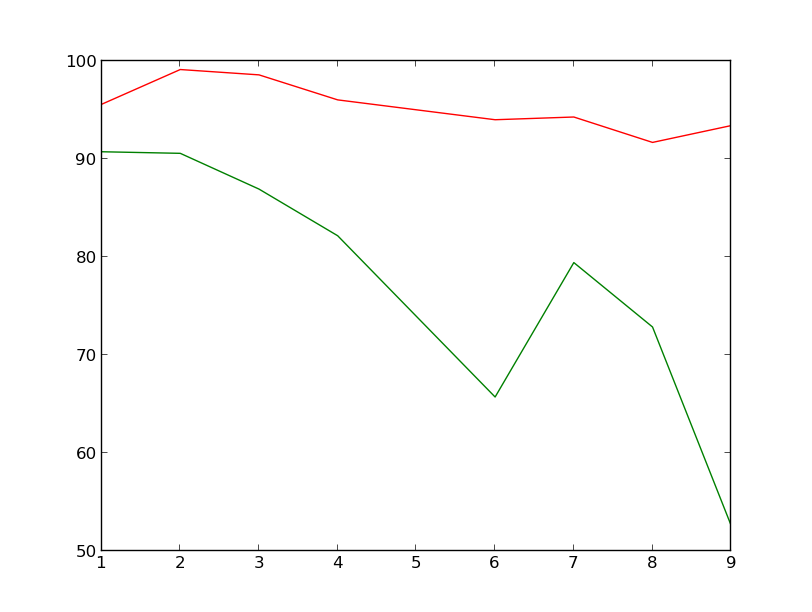
\includegraphics[width=0.8\textwidth]{images/kmeans_2_centers.png}
\caption{A plot of the centroids of the clusters discovered through k-means clustering with 2 clusters. x-axis is the features, y-axis is score (\%)}
\label{fig:kmeans_2_centers}
\end{figure}

\begin{figure}[h!]
\centering
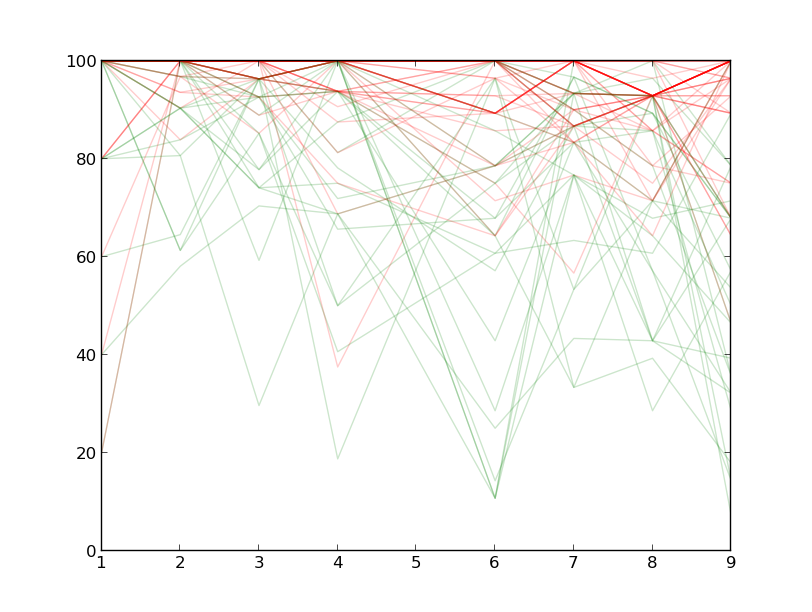
\includegraphics[width=0.8\textwidth]{images/kmeans_2.png}
\caption{A plot of all the students that submitted for each exercise. They are plotted with an opacity of 0.2 and the colours represent the cluster which they belong to after performing k-means cluster with 2 clusters. x-axis is the features, y-axis is score (\%)}
\label{fig:kmeans_2}
\end{figure}

\begin{figure}[h!]
\centering
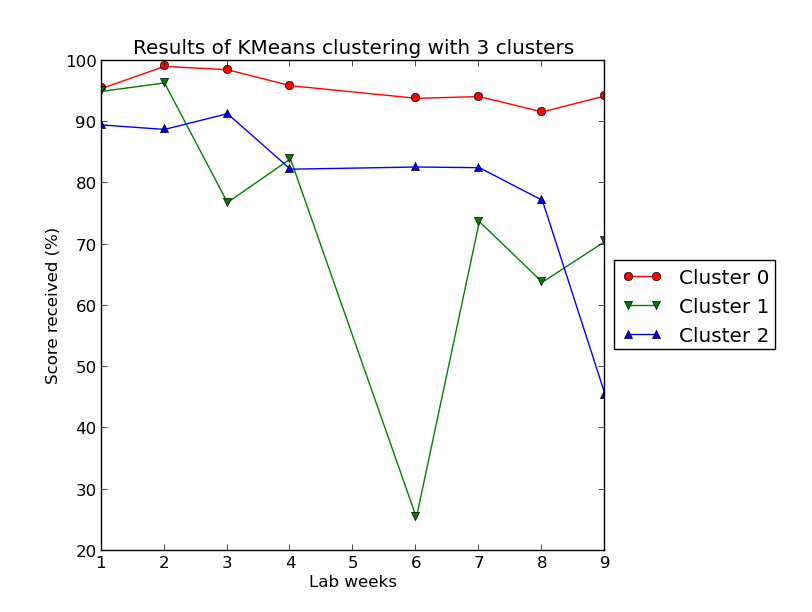
\includegraphics[width=0.8\textwidth]{images/kmeans_3_centers.png}
\caption{A plot of the centroids of the clusters discovered through k-means clustering with 3 clusters. x-axis is the features, y-axis is score (\%)}
\label{fig:kmeans_3_centers}
\end{figure}

\begin{figure}[h!]
\centering
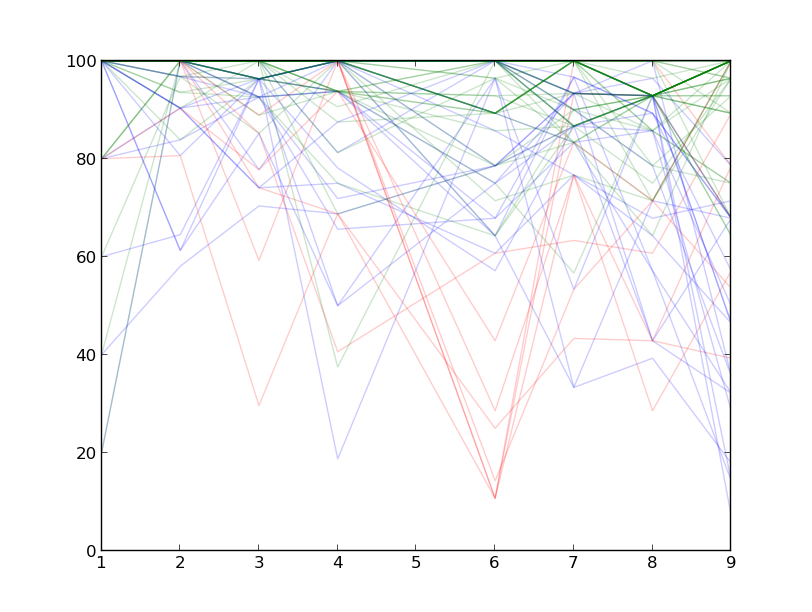
\includegraphics[width=0.8\textwidth]{images/kmeans_3.png}
\caption{A plot of all the students that submitted for each exercise. They are plotted with an opacity of 0.2 and the colours represent the cluster which they belong to after performing k-means cluster with 3 clusters. x-axis is the features, y-axis is score (\%)}
\label{fig:kmeans_3}
\end{figure}

\begin{figure}[h!]
\centering
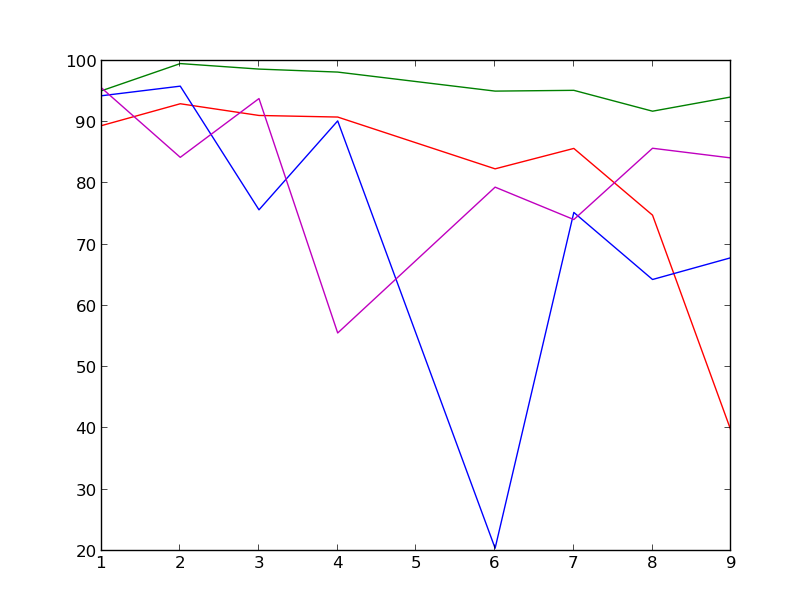
\includegraphics[width=0.8\textwidth]{images/kmeans_4_centers.png}
\caption{A plot of the centroids of the clusters discovered through k-means clustering with 4 clusters. x-axis is the features, y-axis is score (\%)}
\label{fig:kmeans_4_centers}
\end{figure}

\begin{figure}[h!]
\centering
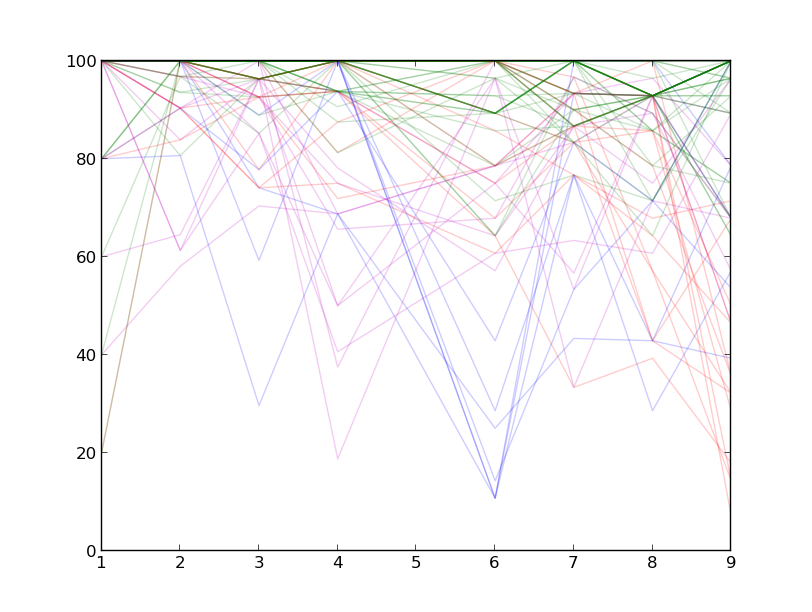
\includegraphics[width=0.8\textwidth]{images/kmeans_4.png}
\caption{A plot of all the students that submitted for each exercise. They are plotted with an opacity of 0.2 and the colours represent the cluster which they belong to after performing k-means cluster with 4 clusters. x-axis is the features, y-axis is score (\%)}
\label{fig:kmeans_4}
\end{figure}


\bibliographystyle{abbrv}
\bibliography{thesis}

\end{document}
